\chapter{Tesztelés}
\label{chap:fejezet5}

\section{Változtatások tesztelésének folyamata, új tesztek felvétele}

A SourceMeter eszközkészlet szoftverjeinek a működését regressziós teszteléssel (röviden regtest) ellenőrizzük. Ez egy olyan tesztelési módszer, amely a változásokat követően újból elvégzi az alkalmazás korábbi tesztjeit annak érdekében, hogy megbizonyosodjon arról, hogy a változtatások nem okoztak olyan hibákat, amelyek hatással lehetnek az alkalmazás teljesítményére.
A célja az, hogy könnyen ellenőrizhető legyen a korábban működő szoftverek új funkciók implementálása után is, és hogy az új funkciók, amelyeket hozzáadtak az alkalmazáshoz, nem okoznak olyan hibákat, amelyek negatívan befolyásolják az alkalmazás teljesítményét. Ezenkívül az alkalmazás megbízhatóságának növeléséhez és a hibák korai észleléséhez.
A regressziós teszteket Pythonban megírt szkriptek segítségével futtatjuk le, melyek korábbi verzióban a SourceMeter szoftvercsomagjainak eszközeinek mindegyikéhez nyelv alapján rendelt egy-egy összefoglaló tesztet. Ezen összefoglaló tesztek a különböző eszközök számára tartalmaz nagy mennyiségben teszteseteket, melyek mindegyikének sikeresen kell lefutnia, hogy a programokban végbevitt fejlesztések el legyenek fogadva.

A tesztek eredményeit korábban, helyesen lefutott tesztek eredményeihez hasonlítjuk futtatás után, és a fennakadó különbségeket feltüntetjük '.diff' kiterjesztésű fájlokban. Ennek előnye, és egyben hátránya, hogy minden eltérésről értesül a fejlesztő tesztelés során, súlyosságtól függetlenül. Az eredmények vizsgálata során a fejlesztőnek kötelessége eldönteni, hogy a kimutatott eltérések ténylegesen hibák vagy hamis pozitívak.

\begin{figure}[!htbp]
    \caption{Példa .diff fájl}\label{fig:difffile}
    \centering
    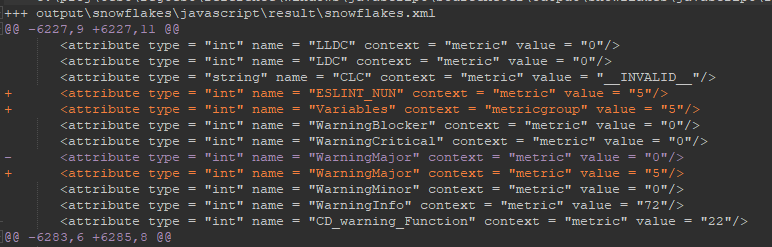
\includegraphics[width=0.9\textwidth]{diffpelda.png}
\end{figure}

Ezek a tesztek minden implementált változtatás után futtatva vannak, lokális számítógépen és Jenkins használatával központi szerveren. 
A Jenkins egy nyílt forráskódú, Java alapú, folytonos integrációs (Continous Integration, avagy CI) és folytonos szállítási (Continous Delivery, avagy CD) eszköz, amely lehetővé teszi a szoftvertervezők számára, hogy hatékonyan és automatizáltan integrálják, teszteljék és kézbesítsék az alkalmazásaikat. Ez alapvetően egy központi szerveren van futtatva, amely képes összekapcsolni és koordinálni a különböző forrásokat és eszközöket, például verziókezelő rendszereket, építőrendszereket és tesztelő keretrendszereket.

\section{Regressziós tesztek módosítása}

Ezeknek a statikus teszteknek volt egy olyan hiányossága, mely munkavégzés során nagyon sok időbe telt és jelentős frusztrációt okozott. A program elemzői adott nyelvekre csak egy fordítási célponttal (build targettel) rendelkeztek. Ez azt jelentette, hogy ha például egy adott részét akarnánk ellenőrizni a szoftvercsomagunknak, például csak az ESLintRunnert, ahhoz a teljes SourceMeter-JavaScriptet kellett tesztelnünk, mert célpont nem volt definiálva. Ezeknek során azon kívül hogy "feleslegesen" teszteltük a programot fejlesztés során, jelentősen sok időbe telt az egyes futtatások végbemenetele, alkalmanként akár több órába is. Emellett olyan esetekben, amikor saját eszközön teszteltem, a build folyamat erőforrásigénye modern rendszereket is le tud terhelni annyira, hogy használhatatlan legyen a teszt buildelése és futtatása során, megállítva a fejlesztési folyamatot.
Megoldásként az SourceMeter összes támogatott nyelvének összes programjához létrehoztam külön-külön tesztelési célpontokat, melyek során csak az adott teszthez szükséges alprogramokat és függőségek fordultak le.

\begin{lstlisting}[caption={CMake célpontok JavaScript teszteléshez},label={lst:abs-computedfiltering}, style={CStyle}]
create_run_regtest_target(javascript_all AN-JavaScript GenealogyTool)
create_run_regtest_target(javascript_jsan jsan_virtual_target)
create_run_regtest_target(javascript_jsan2lim jsan_virtual_target JSAN2Lim)
create_run_regtest_target(javascript_eslintrunner eslintrunner_virtual_target ESLint2Graph)
create_run_regtest_target(javascript_eslint2graph jsan_virtual_target JSAN2Lim eslintrunner_virtual_target ESLint2Graph GraphDump)
create_run_regtest_target(javascript_duplicatedcodefinder AN-JavaScript GenealogyTool)
...
\end{lstlisting}
    
Első lépésként a teszteléshez tartozó CMakeList fájlban kellett módosításokat hozni. Új célpontok létrehozása önmagában egyszerű, mert már definiált funkciók segítségével lehet létrehozni. A nehezebb része ennek a lépésnek az adott programokhoz tartozó függőségek kikeresése és hozzáadása az adott célpontokhoz. Legtöbb esetben ez egyszerű volt, mivel adott programokhoz név alapján volt rendelve CMake target, míg másoknál meg némi eltéréssel, de követhető módon. JSAN esetén például "jsan\_virtual\_target" volt megadva, azt jelezve, hogy nem kizárólag a JSAN volt csak fordítva ennek meghívásával, hanem egyszerre több minden, melyek szükségesek voltak helyes működéshez. Ezek kikutatása a meglévő tesztek alapján könnyen elvégezhető volt, tesztek során használt programok alapján rendeltem hozzá az adott függőségeket a célpontokhoz. Emellett adott nyelvek esetén, mint Java vagy C++, egyéb függőségek megadása is szükséges volt. Mivel a programokhoz nem volt kellő dokumentáció, mely részletezné a kellő függőségeket sikeres fordításhoz, ezek kikutatásához a fordítás során megjelenő hibák alapján adtam meg a különböző célpontokhoz a szükséges modulokat. 

Ezután az új teszteseteket a teszteket futtató python szkripten belül is definiálni kellett.
Ennek a lépésnek nagy része tömbök létrehozásából és argumentumokhoz új választható lehetőségek felvételéből állt. A tömbök a különböző, futtatandó teszteket tartalmazta, melyek közül a "\_all" utótaggal rendelkezők tartalmazták az adott nyelvnek összes tesztét, míg a többi, melyek program nevekkel voltak ellátva, csak az adott program tesztjét futtatta.

\begin{figure}[!htbp]
    \caption{JavaScript regressziós tesztjeit tartalmazó objektumok}\label{fig:testcases}
    \centering
    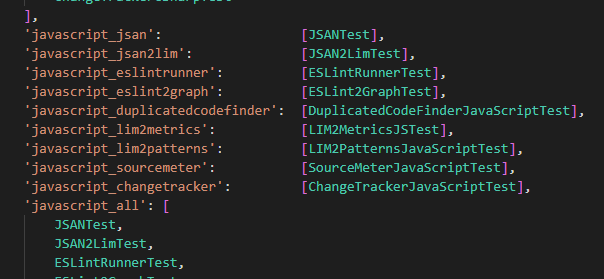
\includegraphics[width=0.9\textwidth]{testcases.png}
\end{figure}

Adott helyeken még szükséges volt módosítani ahhoz, hogy akadásmentesen futhassanak a tesztek. Java tesztek esetén ellenőrizni kellett a "JAVA\_HOME" környezeti változóra, hiszen hiányában ezek a tesztek nem futnak le. Emellett Python teszteknél futásidőben ellenőrzi a program dinamikusan, hogy megfelelő verzióval rendelkezünk-e, mivel futásidő közben telepíti a teszt az elemzéshez szükséges "pylint" szoftvert.
Ezek ellenőrzéséhez létrehoztam külön tömböket, melyek tartalmazzák a nyelvekhez tartozó teszteket szöveg formátumban, mivel a paraméterként kapott teszteket is ilyen formátumban kezeljük.
A teszteket, amiket megadhatunk paraméterként, hozzáadtam a megfelelő argumentumhoz. Mivel nem akartam hogy egy hosszú sor, vagy egy nagy, nehezen olvasható szövegblokk legyen, nyelvenként csoportosítva, tagolva adtam meg ezeket.

Ezek után a módosítások után még fennállt egy probléma. Minden teszt futtatása esetén (Regtest\_all futtatása) minden teszt kétszer futott le. A teszteknek a tömbjei egy 'all\_tests' nevű szótárban (dictionaryben) vannak megadva. Tesztek futtatása során ellenőrizzük hogy adott nyelvhez tartozik-e az éppen iterált teszt, ha nem, akkor kihagyjuk annak futtatását. Mivel a tesztek külön-külön meg voltak adva a programokra és nyelvekre, így alapesetben minden teszt kétszer futott volna le. Ennek megoldására legegyszerűbb módszer a duplikált tesztek törlése volt abban az esetben, ha 'Regtest\_all' futtatása volt a feladat, azaz minden, nyelvhez tartozó összetett tesztet töröltünk az 'all\_tests'-ből. 


\begin{lstlisting}[caption={CMake célpontok JavaScript teszteléshez},label={lst:abs-computedfiltering}, language={Python}]
if LANG == "all":
    del all_tests['cpp_all']
    del all_tests['csharp_all']
    del all_tests['java_all']
    del all_tests['javascript_all']
    del all_tests['rpg_all']
    del all_tests['python_all']
\end{lstlisting}